\documentclass[11pt]{article}

\usepackage[margin=1in]{geometry}
\usepackage[T1]{fontenc}
\usepackage{lmodern}
\usepackage{microtype}
\usepackage{graphicx}
\usepackage{subcaption}
\usepackage{booktabs}
\usepackage{siunitx}
\usepackage{xcolor}
\usepackage{float}
\usepackage{hyperref}

\sisetup{
  table-number-alignment = center
}

\hypersetup{
  colorlinks=true,
  linkcolor=blue!50!black,
  citecolor=blue!50!black,
  urlcolor=blue!50!black
}

\setlength{\parskip}{0.6em}
\setlength{\parindent}{0pt}

\title{\textbf{CAA v3 Sweep Summary}}
\author{}
\date{May 2026}

\begin{document}

\maketitle

\section{Overview}

This report summarizes the CAA v3 sweep over steering coefficient and steered layer on the abstention benchmark suite for \texttt{Qwen 2.5 0.5B}, \texttt{Qwen 2.5 1.5B}, \texttt{Qwen 2.5 3B}, \texttt{Qwen 2.5 7B}, and \texttt{Tulu 3.1 8B}.

For each model, the selected configuration is the tested layer-coefficient pair with the highest mean F1 across the suite. Precision and recall are reported at that same operating point. Recall is the fraction of abstention-worthy examples on which the model abstains. Precision is the fraction of abstentions that are correct. F1 summarizes the balance between the two.

Some coefficient-model combinations have no reported result. In this sweep, that means the model collapsed at that coefficient for every tested layer: the benchmark hit the 4-hour timeout and the model entered repeated gibberish loops. Missing points should therefore be read as collapse, not as untested settings.

\section{Best tested configurations}

Table~\ref{tab:best-configs} summarizes the best tested setting for each model. The best F1 values occur at coefficients 2 or 3 for all models and at layers 14--19. \texttt{Qwen 2.5 1.5B} attains the highest mean F1, while \texttt{Qwen 2.5 7B} has the highest precision at its own best-F1 setting.

\begin{table}[H]
\centering
\caption{Best tested configuration for each model.}
\label{tab:best-configs}
\begin{tabular}{lcc S[table-format=1.4, round-mode=none] S[table-format=1.4, round-mode=none] S[table-format=1.4, round-mode=none]}
\toprule
Model & Coeff. & Layer & {Precision} & {Recall} & {F1} \\
\midrule
Qwen 2.5 0.5B & 2.0 & 14 & 0.5567 & 0.8460 & 0.6455 \\
Qwen 2.5 1.5B & 2.0 & 15 & 0.5556 & 0.9369 & 0.6709 \\
Qwen 2.5 3B   & 3.0 & 19 & 0.5492 & 0.8469 & 0.6315 \\
Qwen 2.5 7B   & 2.0 & 16 & 0.6047 & 0.6288 & 0.5825 \\
Tulu 3.1 8B   & 3.0 & 16 & 0.5723 & 0.6154 & 0.5543 \\
\bottomrule
\end{tabular}
\end{table}

\begin{figure}[H]
\centering

\includegraphics[width=0.92\textwidth]{max_f1_vs_model_scale.png}
\caption{Peak mean F1 for each model at its best tested layer-coefficient pair.}
\label{fig:best-f1}
\end{figure}

\section{Effect of coefficient}

The best F1 for every model is reached at coefficient 2 or 3. At larger coefficients, F1 declines when evaluation completes, and some models have no reported value because all layers collapse at that coefficient. In this sweep, increasing the coefficient beyond the moderate range did not improve the best observed operating point.

\begin{figure}[H]
\centering

\includegraphics[width=0.92\textwidth]{f1_trajectory_best_layer.png}
\caption{F1 by steering coefficient at the best tested layer for each model. Missing values indicate collapse at that coefficient across all tested layers, identified by benchmark timeout at 4 hours and repeated gibberish loops in generation.}
\label{fig:trajectory}
\end{figure}

\section{Precision-recall trade-offs}

A tested setting is Pareto dominated if another tested setting for the same model is at least as good on both precision and recall and strictly better on one of them. The Pareto frontier is the set of settings that remain after removing dominated points. Figure~\ref{fig:pareto} therefore shows, for each model, the best precision-recall trade-offs reached anywhere in the sweep.

\begin{figure}[H]
\centering

\includegraphics[width=0.92\textwidth]{pr_tradeoff_pareto.png}
\caption{Precision-recall Pareto frontiers for the tested settings.}
\label{fig:pareto}
\end{figure}

The frontier for \texttt{Qwen 2.5 1.5B} extends furthest into the high-recall region while remaining competitive on precision. \texttt{Qwen 2.5 7B} occupies a higher-precision, lower-recall region, and \texttt{Tulu 3.1 8B} spans a narrower range overall. Supporting plots for per-model best-point precision/recall, coefficient trajectories, and representative layer-coefficient heatmaps are included in the appendix.

\section{Summary}

Across the tested models, the strongest settings are concentrated at coefficients 2--3 and layers 14--19. Within this sweep, \texttt{Qwen 2.5 1.5B} attains the highest mean F1, and the larger models do not improve on that peak result.

\appendix

\section{Supporting plots}

\begin{figure}[H]
\centering
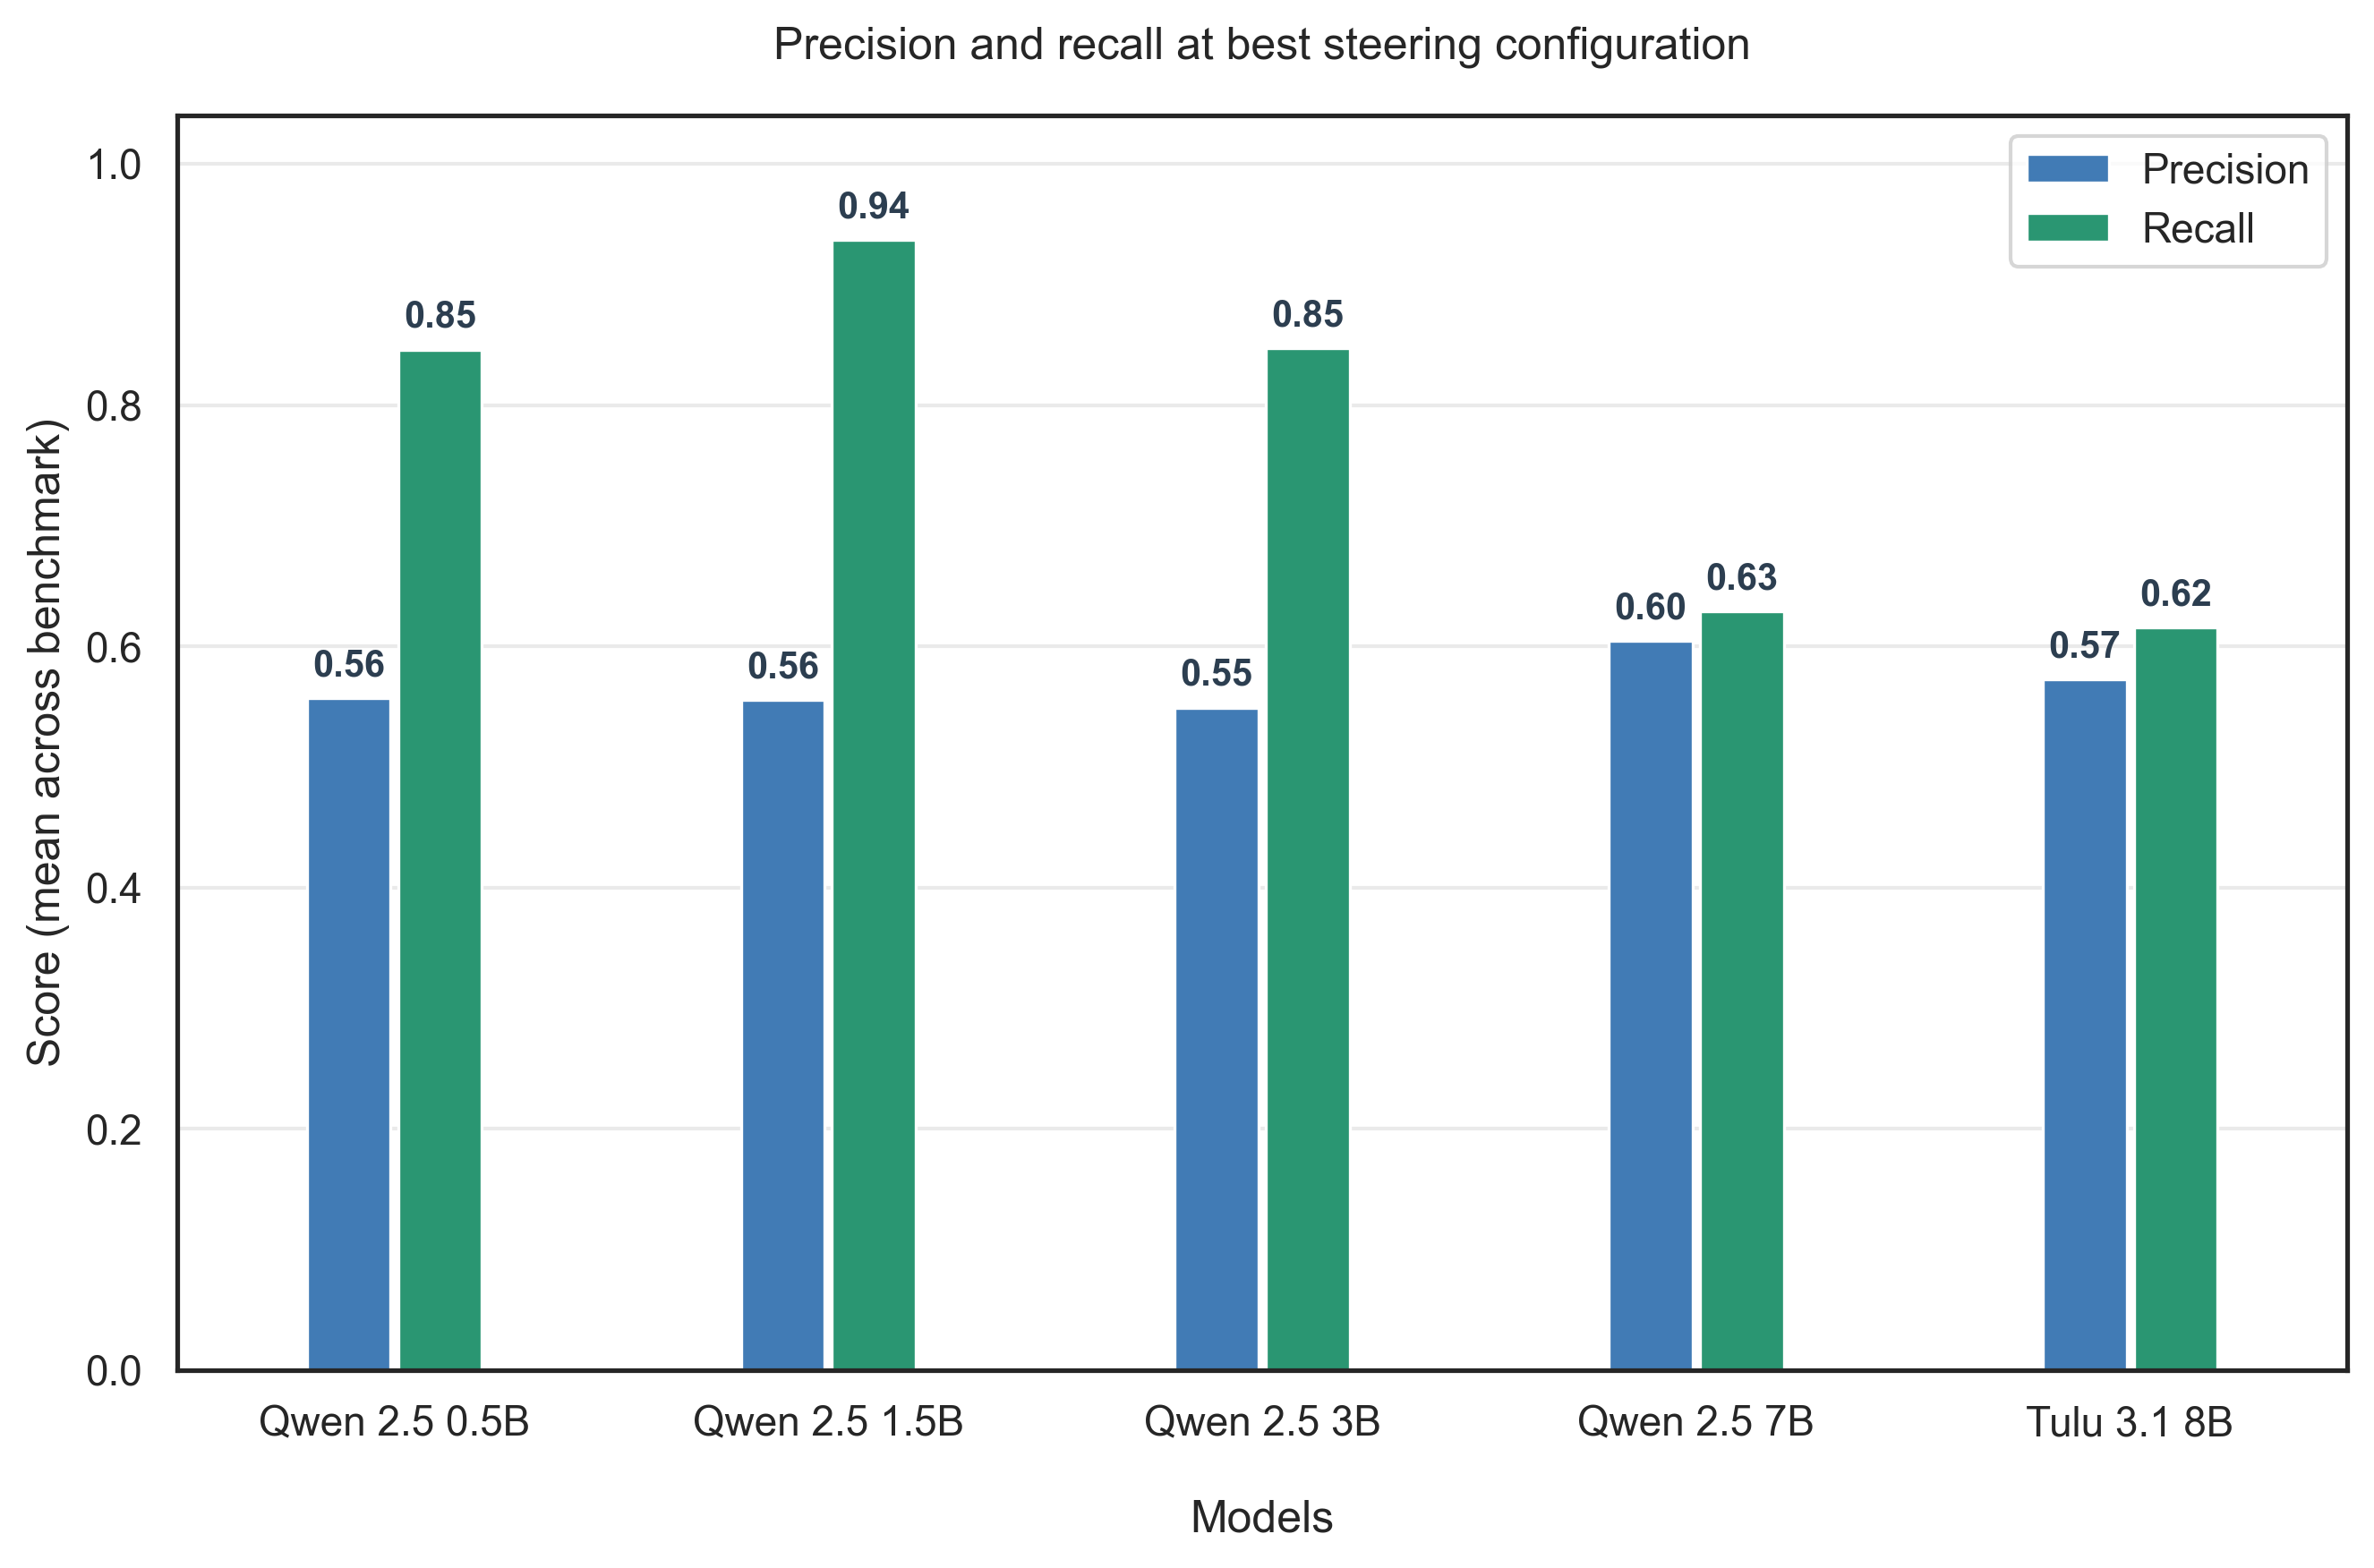
\includegraphics[width=0.92\textwidth]{precision_recall_best_config.png}
\caption{Precision and recall at each model's best tested configuration.}
\label{fig:precision-recall-bars}
\end{figure}

\begin{figure}[H]
\centering
\begin{subfigure}{0.49\textwidth}
    \centering
    
\includegraphics[width=\linewidth]{heatmap_Qwen_2.5_1.5B.png}
    \caption{\texttt{Qwen 2.5 1.5B}}
\end{subfigure}
\hfill
\begin{subfigure}{0.49\textwidth}
    \centering
    
\includegraphics[width=\linewidth]{heatmap_Qwen_2.5_3B.png}
    \caption{\texttt{Qwen 2.5 3B}}
\end{subfigure}

\vspace{0.8em}

\begin{subfigure}{0.49\textwidth}
    \centering
    
\includegraphics[width=\linewidth]{heatmap_Qwen_2.5_7B.png}
    \caption{\texttt{Qwen 2.5 7B}}
\end{subfigure}
\hfill
\begin{subfigure}{0.49\textwidth}
    \centering
    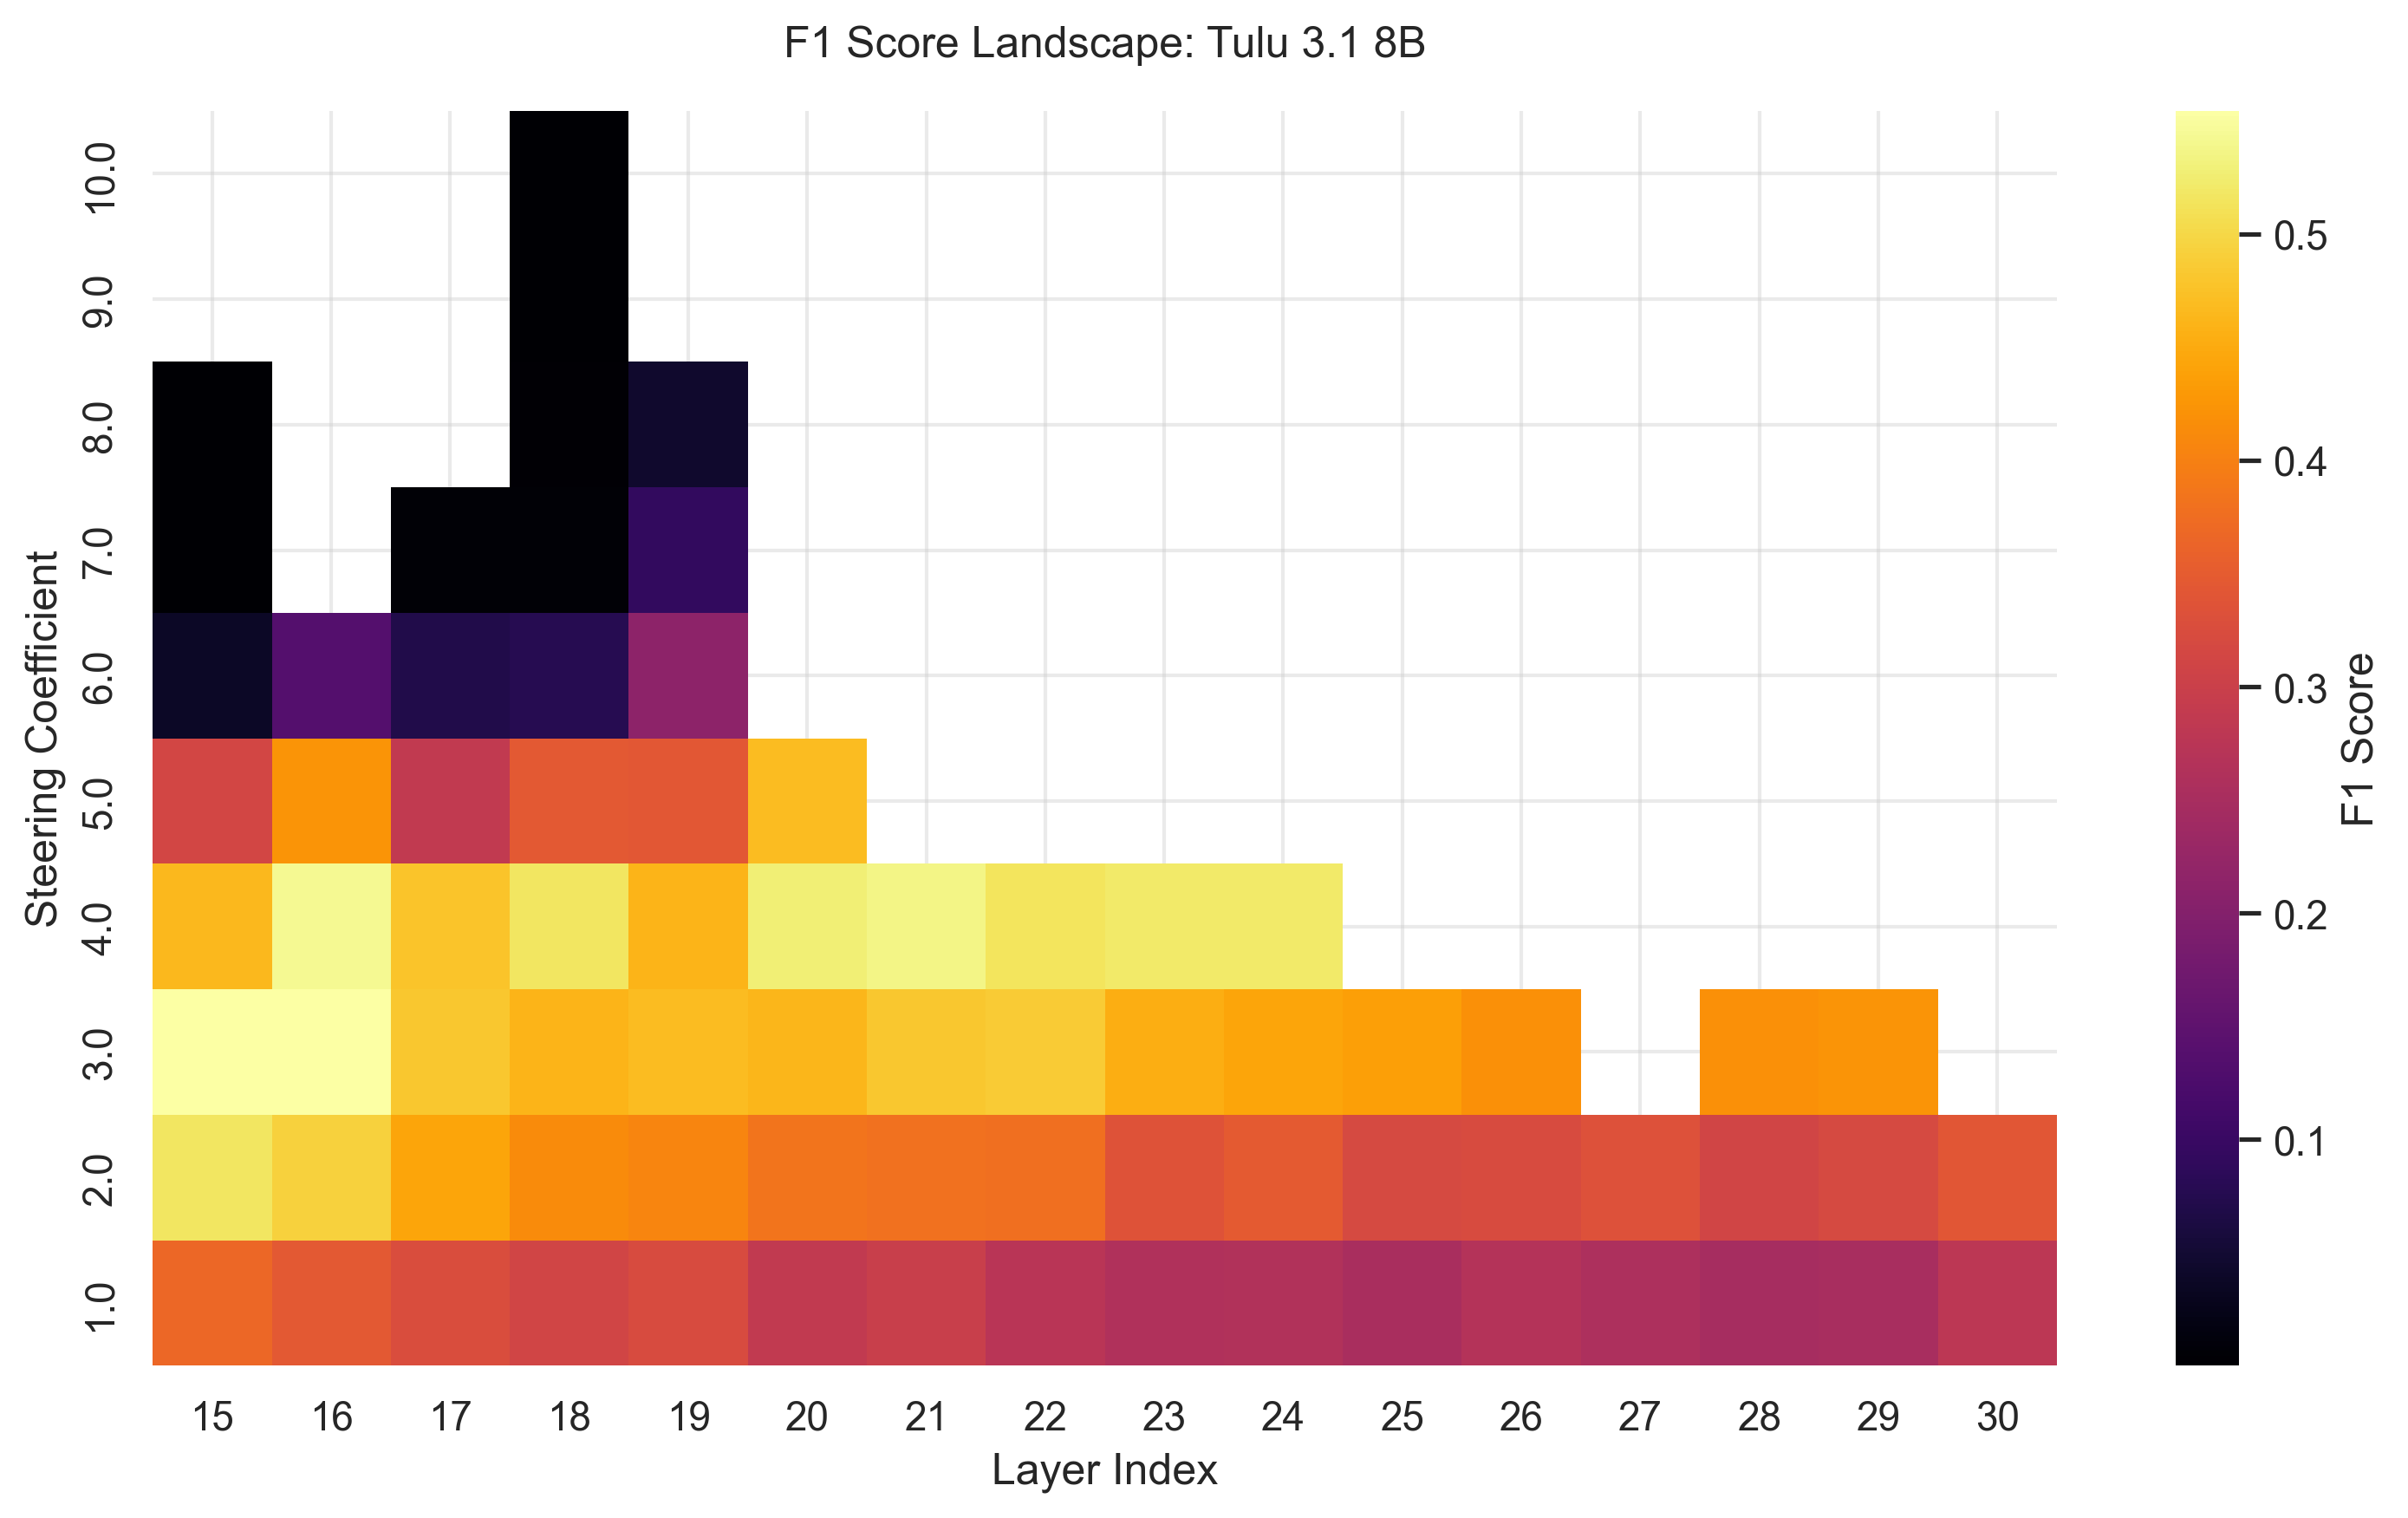
\includegraphics[width=\linewidth]{heatmap_Tulu_3_1_8B.png}
    \caption{\texttt{Tulu 3.1 8B}}
\end{subfigure}
\caption{Representative F1 heatmaps over layer and coefficient. Brighter regions indicate higher mean F1.}
\label{fig:heatmaps}
\end{figure}

\end{document}
